\documentclass[final]{beamer}
\usepackage[utf8]{inputenc}
\usepackage[orientation=portrait,size=a0,scale=1.4]{beamerposter}
\usepackage{amsmath}
\usepackage{amsfonts}
\usepackage{amssymb}
\usepackage{graphicx}
\usepackage{subcaption}

\title{Comportamento de Busca por Caixas em Felidae: Uma Revisão Etológica Integrativa}
\author{Prof. Dr. Ney Lemke}
\institute{Universidade Estadual Paulista (UNESP), Instituto de Biociências, Botucatu, SP}
\date{V Congresso Brasileiro de Proteção, Bem-Estar e Patologia Animal \\ 11 a 15 de agosto de 2025}

\begin{document}

\begin{frame}[t] 
  \maketitle

  \begin{columns}[T]

    \begin{column}{.32\linewidth}
      \begin{block}{Introdução}
        O comportamento de busca por caixas é um padrão robusto e filogeneticamente conservado em Felidae, desde gatos domésticos (\textit{Felis catus}) até grandes felinos. Longe de ser uma curiosidade, este comportamento tem profundas implicações para o bem-estar animal. Esta revisão integrativa sintetiza evidências empíricas da etologia, biologia evolutiva e fisiologia para elucidar suas bases mecanicistas e significado adaptativo, utilizando as quatro questões de Tinbergen (causa, ontogenia, função e filogenia).
      \end{block}
      \begin{block}{Metodologia}
        Foi realizada uma revisão integrativa da literatura, analisando estudos empíricos, observações de campo e análises comparativas. A síntese foi estruturada sob o framework das quatro questões de \citet{tinbergen1963} para fornecer uma análise compreensiva e multi-nível do comportamento, abordando:
        \begin{itemize}
            \item \textbf{Causas Próximas:} Mecanismos fisiológicos e ambientais.
            \item \textbf{Ontogenia:} Desenvolvimento ao longo da vida do indivíduo.
            \item \textbf{Função Adaptativa:} Vantagens de sobrevivência e reprodução.
            \item \textbf{Evolução Filogenética:} História evolutiva do comportamento.
        \end{itemize}
      \end{block}
      \begin{block}{Resultados Principais}
        \begin{itemize}
            \item \textbf{Redução de Estresse:} Caixas funcionam como ferramentas primárias de redução de estresse. Ensaios clínicos randomizados com gatos de abrigos mostraram reduções significativas no Escore de Estresse de Gatos (CSS) e nos níveis de cortisol \citep{vinke2014}.
            \item \textbf{Função Dupla:} Caixas servem a propósitos ofensivos (plataforma de emboscada) e defensivos (refúgio), refletindo a posição trófica intermediária dos felinos.
            \item \textbf{Termorregulação:} Caixas fornecem isolamento térmico, ajudando a compensar a diferença entre a zona termoneutra felina (30–38°C) e a temperatura ambiente típica.
            \item \textbf{Implicações Clínicas:} O fornecimento de caixas em clínicas, abrigos e residências reduz patologias relacionadas ao estresse e acelera a recuperação.
        \end{itemize}
      \end{block}
    \end{column}

    \begin{column}{.32\linewidth}
      \begin{block}{Comportamento Conservado em Felidae}
        \begin{figure}
            \centering
            \begin{subfigure}[b]{0.49\textwidth}
                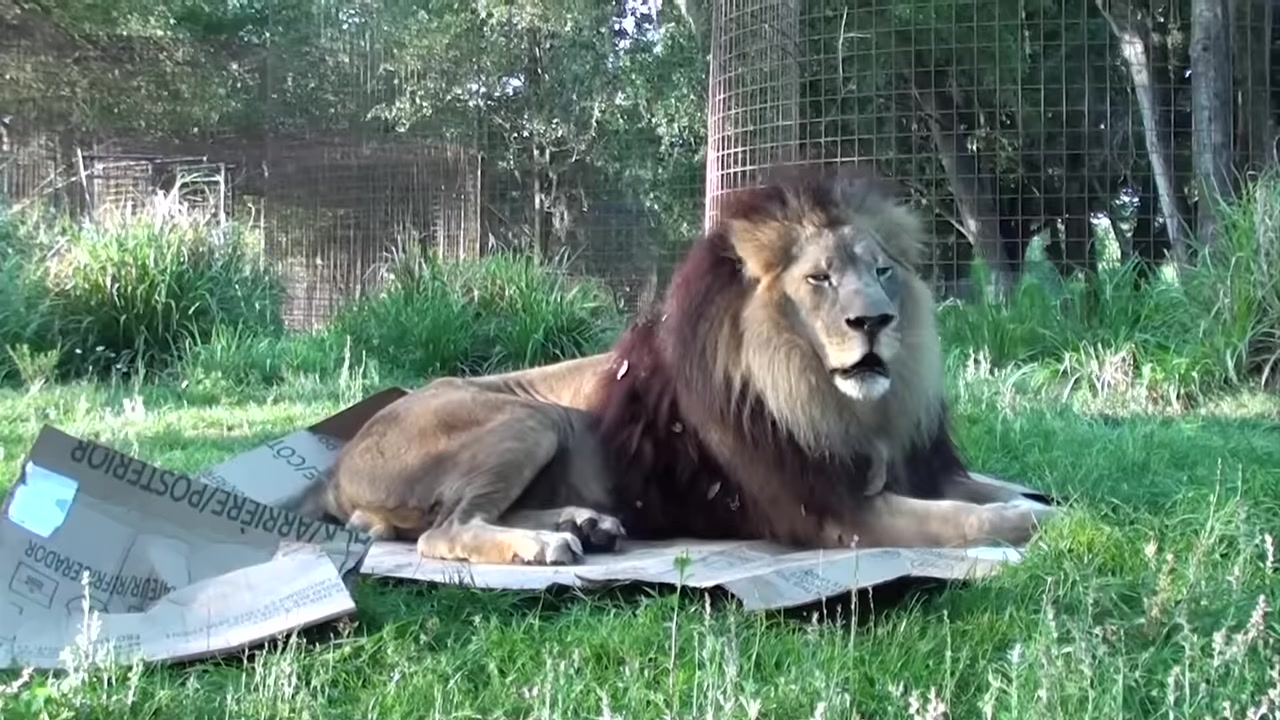
\includegraphics[width=\textwidth]{01_joseph_lion.jpg}
                \caption{Leão}
            \end{subfigure}
            \hfill
            \begin{subfigure}[b]{0.49\textwidth}
                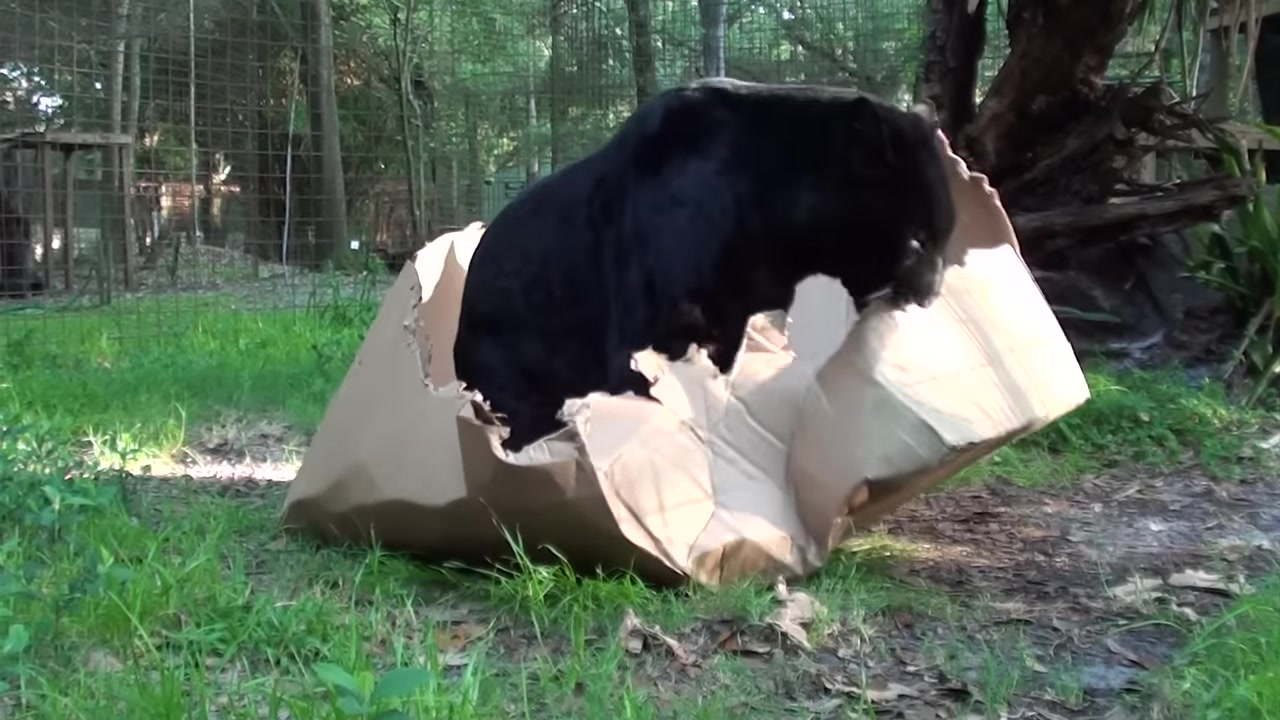
\includegraphics[width=\textwidth]{02_jumanji_panther.jpg}
                \caption{Pantera}
            \end{subfigure}
            
            \vspace{1em}
            
            \begin{subfigure}[b]{0.49\textwidth}
                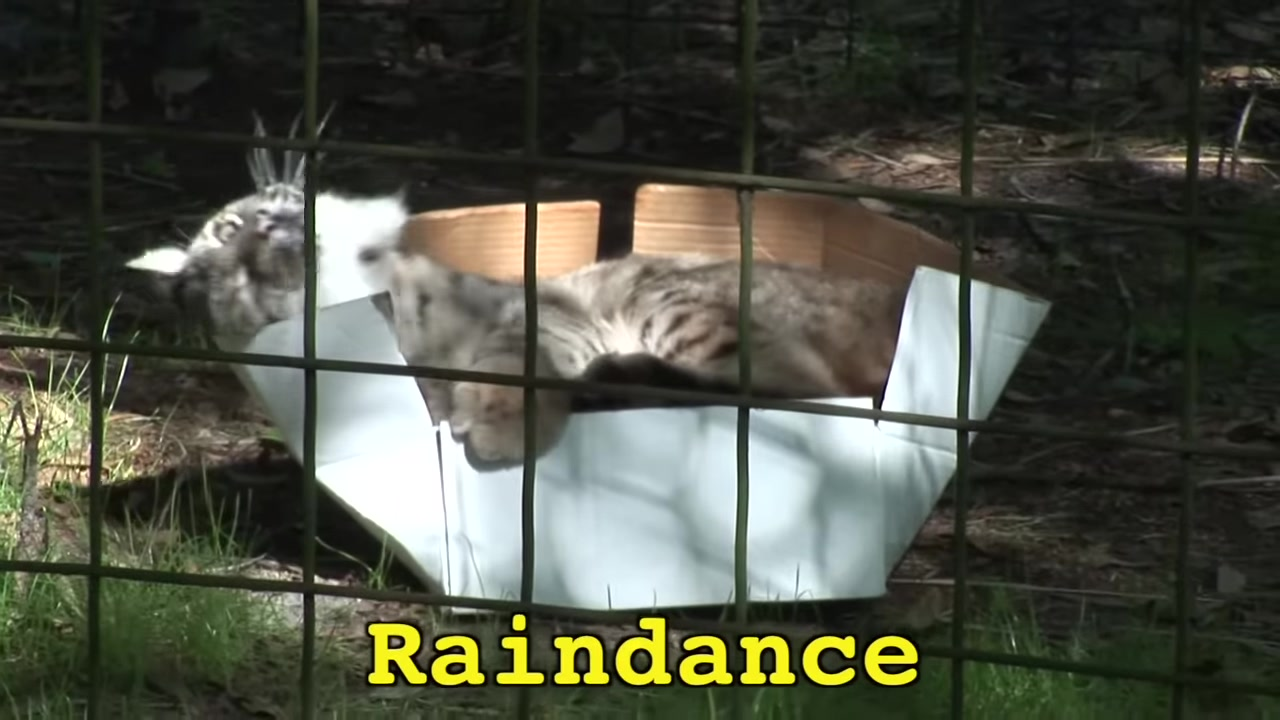
\includegraphics[width=\textwidth]{03_raindance_bobcat.jpg}
                \caption{Lince-pardo}
            \end{subfigure}
            \hfill
            \begin{subfigure}[b]{0.49\textwidth}
                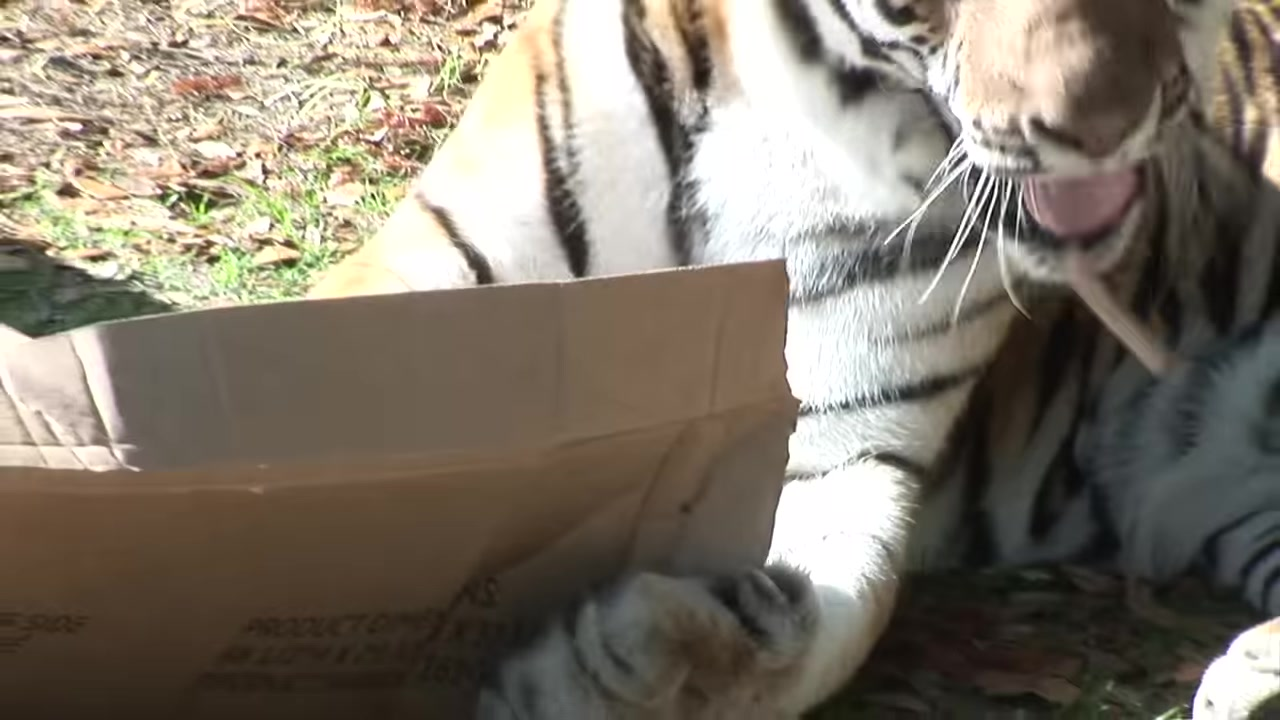
\includegraphics[width=\textwidth]{04_andre_arthur_tigers.jpg}
                \caption{Tigres}
            \end{subfigure}

            \vspace{1em}
            
            \begin{subfigure}[b]{0.49\textwidth}
                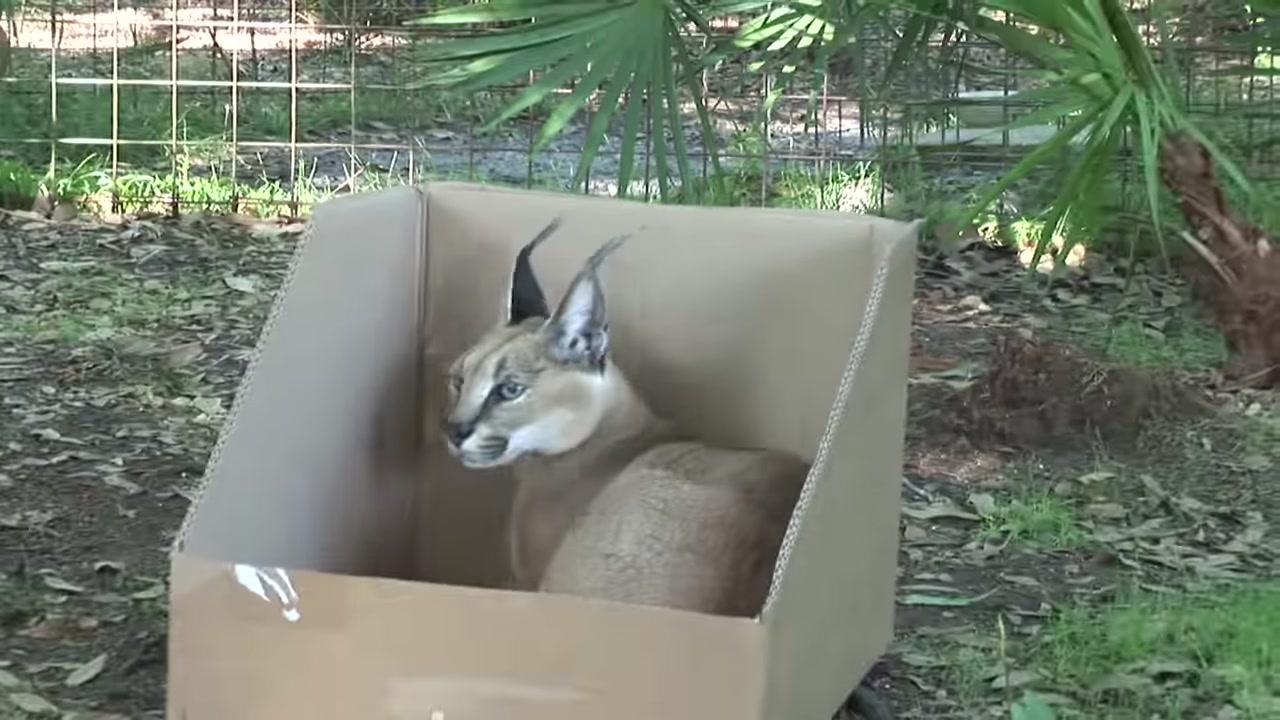
\includegraphics[width=\textwidth]{05_rusty_caracal.jpg}
                \caption{Caracal}
            \end{subfigure}
            \hfill
            \begin{subfigure}[b]{0.49\textwidth}
                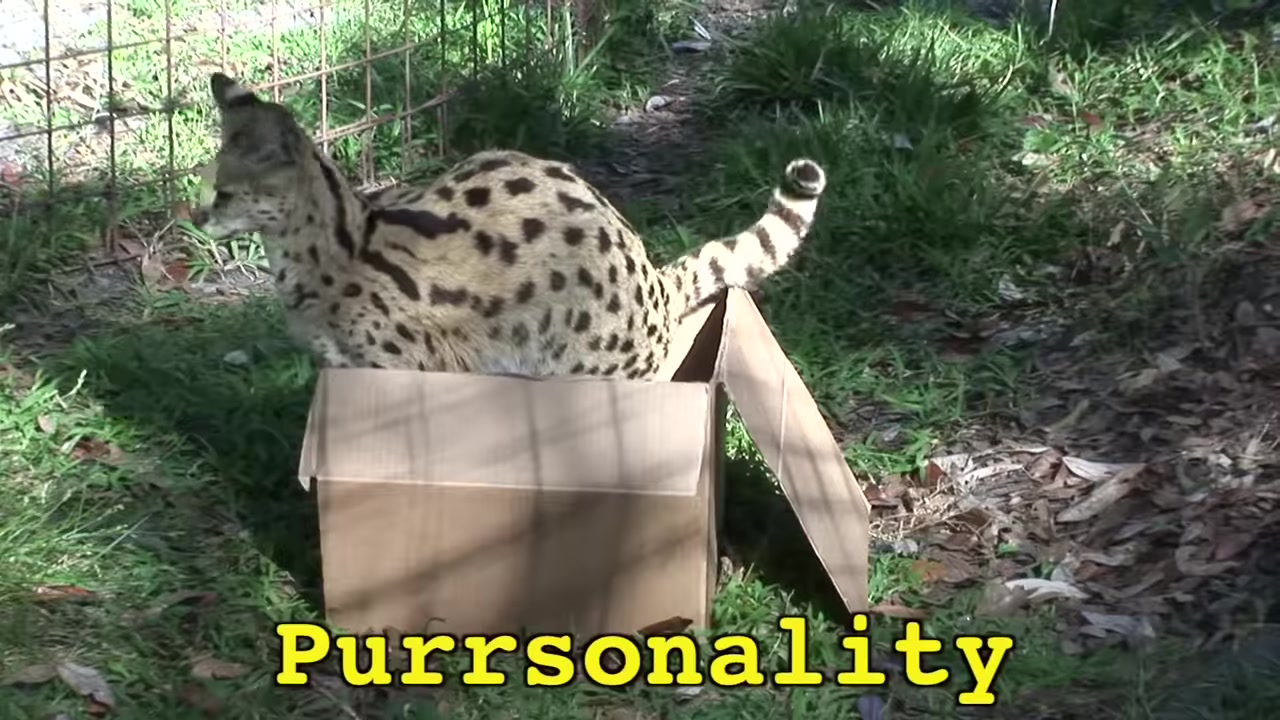
\includegraphics[width=\textwidth]{06_purrsonality_serval.jpg}
                \caption{Serval}
            \end{subfigure}
                        
            \caption{O comportamento de busca por caixas é observado em diversas espécies de felinos, indicando uma forte conservação filogenética. Imagens: \citet{bigcatrescue2019}.}
            \label{fig:felids_in_boxes}
        \end{figure}
      \end{block}
    \end{column}

    \begin{column}{.32\linewidth}
      \begin{block}{Conclusão}
        O comportamento de busca por caixas é uma necessidade etológica fundamental com profundas implicações para o bem-estar felino. Ele serve como uma ferramenta de redução de estresse, uma adaptação para caça e defesa, e um auxílio na termorregulação. A provisão de caixas e esconderijos deve ser considerada um requisito básico de bem-estar em ambientes domésticos, clínicos e de abrigos, respeitando a herança evolutiva dos felinos. Longe de ser uma trivialidade, entender este comportamento é essencial para melhorar a qualidade de vida dos felinos sob cuidado humano.
      \end{block}
      \begin{block}{Referências}
        \begin{itemize}
            \item \footnotesize \textbf{Big Cat Rescue. (2019).} Cats vs Boxes: The Epic Battle! \textit{YouTube}. \url{https://www.youtube.com/watch?v=J11uu8L8FTY}
            \item \footnotesize \textbf{Tinbergen, N. (1963).} On aims and methods of Ethology. \textit{Zeitschrift für Tierpsychologie}, 20(4), 410-433.
            \item \footnotesize \textbf{Vinke, C. M., et al. (2014).} Will a hiding box provide stress reduction for shelter cats? \textit{Applied Animal Behaviour Science}, 160, 86-93.
        \end{itemize}
      \end{block}
    \end{column}

  \end{columns}
\end{frame}

\end{document}
